
\definecolor{red}{rgb}{1,0,0} % 255,0,0
\definecolor{green}{rgb}{0,.8,0.05} % 0,203,14
\begin{tabular}{ll}
	\parbox{9.5cm}{
 		\textbf{Gegeninduktion} ($M_{\textcolor{red}{X}\textcolor{green}{Y}}; \textcolor{red}{X}$: Wirkung,
 		$\textcolor{green}{Y}$: Ursache)\\
		\begin{tabular}{ll}
  		Gegeninduktivit\"at
  			& $M_{21} = \frac{\Psi_{m21}}{i_1} =$ (Meist $= \frac{N_2
  			\phi_{m21}}{i_1}$)\\ 
  			(wenn $\mu$ = const.) & $M = k \cdot \sqrt{L_1 L_2} = M_{21} = M_{12} $  \\
  			Gegeninduktionsspannung
  			& $u_{21} = \dot{\Psi}_{21} = M_{21} \frac{di_1}{dt}$    
		\end{tabular}}
	& \parbox{8.5cm}{
	  	Durchsetzt das sich \"andernde Magnetfeld einer stromdurchflossenen Spule
	  	eine zweite Spule, so wird auch in dieser eine Spannung
	  	(=Gegeninduktionsspannung) induziert.}\\
\parbox{9.5cm}{
		\vspace{.2cm}
  		\textbf{Transformatorgleichungen}\\
		\fbox{$u_1 = L_1 \dfrac{di_1}{dt} \textcolor{red}{+}\textcolor{green}{-}M_{12} \dfrac{di_2}{dt} 
			= L_1 \dfrac{di_1}{dt} \textcolor{red}{-}\textcolor{green}{+}M_{12} \dfrac{di_b}{dt}$} $\qquad$ 
		\fbox{$u_2 = L_2 \dfrac{di_2}{dt}
		\textcolor{red}{+}\textcolor{green}{-} M_{21} \dfrac{d i_1}{dt} 
			= -L_2 \dfrac{di_b}{dt} \textcolor{red}{+}\textcolor{green}{-} M_{21}
			\dfrac{d i_1}{dt}$} 
		\vspace{.2cm}
  			
	  		\textbf{Idealer Trafo}\\ 
	  		\fbox{$"u = \dfrac{u_1}{u_2} = \dfrac{N_1}{N_2} = n$} $\qquad$ (im Leerlauf: $\dfrac{1}{"u} = k \sqrt{\dfrac{L_2}{L_1}}$)
	  		}
  		& \parbox{5cm}{
	  		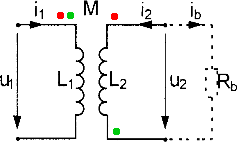
\includegraphics[width=4cm]{bilder/trafo-kopplung.png} \\
      		\small{\textcolor{red}{Gleichsinnig} / \textcolor{green}{Gegensinnig}}} \\
	  		
  	\parbox{9.7cm}{
      		\textbf{Verlustbehafteter Trafo}
      		\begin{list}{$\bullet$}{\setlength{\itemsep}{0cm} \setlength{\parsep}{0cm} \setlength{\topsep}{0cm}} 
              \item Prim\"arstrom im Leerlauf: $L_H$
	          	(ideal $L_H \rightarrow \infty)$
	          \item Hysterese- \& Wirbelstromverluste: $R_{Fe}$
	          	(ideal: $R_{Fe}
	          \rightarrow \infty$) 
	          \item Kupferwiderst\"ande: $R_{Cu1}, R_{Cu2}$
	          	(ideal: $R_{Cu}
	          \rightarrow 0$)
	          \item Streufluss (Kopplung): $L_{\sigma1}, L_{\sigma2}$
	          	(ideal: $L_{\sigma} \rightarrow 0$)
            \end{list}
      		}
  		& \parbox{8.8cm}{
	  		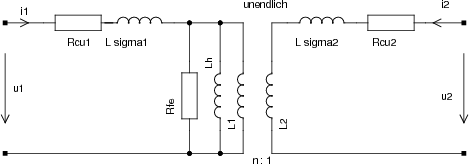
\includegraphics[width=8.8cm]{bilder/trafo-verluste.png}}
   	\end{tabular}